% Single submission for the NeurIPS 2026 workshop on Evaluation of Interactive Agents (IAEval).
% 4 pages excluding references, double blind, non-archival.
%
% TODO before submission
%   [ ] swap this preamble for neurips_2026.sty (anonymous mode, NOT [final]) and refit
%   [ ] check no de-anonymising string survives: names, institution, repo URL, arXiv id
%   [ ] declare the overlap with the conference version in the submission form
%
% Every number comes from data/ via scripts/atlas_tables.py and scripts/probe_tables.py.
% Nothing in this document should be typed by hand.
\documentclass[11pt]{article}
\usepackage[margin=1in]{geometry}
\usepackage{amsmath}
\usepackage{booktabs}
\usepackage{graphicx}
\usepackage{microtype}
\usepackage{natbib}
\usepackage[hidelinks]{hyperref}
\graphicspath{{../figures/}}
\renewcommand{\arraystretch}{1.05}

\newcommand{\ORACLEOBSMEAN}{24.7}
\newcommand{\ORACLEOBSN}{four}

\title{Is It the Game or the Agent?\\
       Measuring What a Game Hides, and Diagnosing Why an Agent Stops Improving}
\author{Anonymous submission}
\date{}

\begin{document}
\maketitle

\begin{abstract}
A win rate is only as informative as what it was measured against, and two things are almost never
measured: how much the game actually hides, and what an agent's plateau is made of. We supply both.
First, an atlas: across 88 games from two engines we compute the bits of hidden information at a
typical decision. Two-player card games saturate early, with a median of 3.1 bits and only two of
23 hiding more than Gin Rummy's 30.1; everything clearly above sits at a larger table, where extra
bits come from extra hands rather than a deeper duel. The atlas also catches its own instrument
lying in two directions: the resampling estimator returns a saturated constant for three games and
a confident \emph{zero} for a game with 30.1 bits. And it exposes a blind spot: of 19 board games,
the only six we can measure are the perfect-information controls, so every fog-of-war game in the
atlas is unmeasured. Second, three probes that turn a plateau against a fixed expert into a
diagnosis. On a Gin Rummy case study they agree: capacity is not the limit (every encoder lands in
21.2 to 30.0 percent), the value of hidden information is bounded but confounded, and an
oracle-observation learner handed the opponent's hand outright reaches \ORACLEOBSMEAN{} percent
against a \textbf{25.5} baseline, a range strictly inside the baseline's. Measuring the domain and
diagnosing the agent are one workflow, and we release the code and all measurements.
\end{abstract}

\section{Two measurements nobody makes}

Agents in imperfect-information games are graded against references that cannot bear the weight.
Random play yields numbers near 99 percent that barely move as the agent improves. Self-play yields
numbers near 50 percent by construction. A pool of past checkpoints moves as the agent moves, so
progress against it is not progress in any absolute sense. Fixing the reference is the obvious
repair, and it is not enough, because two questions survive it.

\textbf{How much does this game hide?} Games are chosen by reputation. Poker is hard, Hanabi is
cooperative, Stratego is big. The quantity that supposedly unites them is rarely computed, so
comparative claims about difficulty rest on tradition.

\textbf{What is the plateau made of?} An agent that stops improving is stuck either because it
cannot see enough (information-bound) or because it can and fails to exploit it (learning-bound).
These call for opposite work, and one win rate cannot separate them.

We answer the first by measurement and the second by three probes, and the case study shows why
they belong in the same paper: without the atlas, a plateau invites the excuse that the game hides
too much; without the probes, the atlas is a table nobody acts on.

\section{Part I: an atlas of what is hidden}

Hidden information at a decision is $\log_2$ of the number of histories consistent with the acting
player's information state. Zero is perfect information; each further bit doubles the worlds the
player must consider. We compute it three ways and always report which.

\textbf{Exact} enumeration walks the tree and groups histories by information state. This is ground
truth, and it is affordable on 11 of our 88 rows. \textbf{Closed form} counts the ways the hidden
hands could have been dealt: $\log_2\binom{u}{k}$ for one hidden hand out of $u$ unseen cards, and
the multinomial for a full table, since it matters which opponent holds which cards. It is exact
arithmetic but counts hands only, ignoring what public cards have ruled out, so it overestimates
mildly; Leduc sizes that gap at 2.01 exact against 2.30 closed form. \textbf{Resampling} draws
worlds consistent with the information state and counts the distinct ones, censored at the sample
count.

The catalog spans 79 games from OpenSpiel \citep{openspiel}, the only engine here exposing
information-state strings and world resampling, and 9 from RLCard \citep{rlcard} for games OpenSpiel
does not ship, Mahjong and UNO above all. Gin Rummy is deliberately measured by both so the closed
form can be cross-checked across libraries; it agrees at 30.1 bits each. PettingZoo
\citep{pettingzoo} supplies the environment API for the case study.

\begin{table}[t]
  \centering \small
  % generated by scripts/make_tables.py -- do not edit by hand
\begin{tabular}{l r r r l}
\toprule
Family & Games & Measured & Median bits & Range \\
\midrule
Card games, 2p & 23 & 18 & 3.1 & 0.0 to 32.9 \\
Gin Rummy dial & 8 & 8 & 16.6 & 5.1 to 30.1 \\
Card games, 3-4p & 21 & 15 & 39.9 & 2.6 to 109.6 \\
Dice games & 6 & 6 & 6.5 & 2.6 to 12.9 \\
Bargaining and signalling & 8 & 5 & 1.0 & 0.7 to 4.5 \\
Board and fog of war & 19 & 6 & 0.0 & 0.0 to 0.0 \\
Solo against chance & 3 & 0 & n/a & n/a \\
\bottomrule
\end{tabular}

  \caption{The atlas by family. \emph{Measured} is how many games in the family admit any estimate
  at all, which is as informative as the bits: the board family's six measured games are precisely
  its perfect-information controls, so every fog-of-war game is unmeasured.}
  \label{tab:families}
\end{table}

\paragraph{Two-player card games saturate.} Their median is 3.1 bits, and of 23 only two hide more
than standard Gin Rummy's 30.1: bridge uncontested bidding at 32.9 and, unexpectedly, UNO at 33.9.
A 52-card deck split between two hands cannot conceal much more. A difficulty ladder assembled from
distinct two-player card games therefore bunches at the top rather than spanning a range.

\paragraph{More hidden information means more players.} The three and four-handed family has a
median of 31.1 bits and reaches 163.4 for Mahjong, with Hearts, Spades and contract bridge at 56.2.
Those bits are bought with extra hands and arrive attached to coalitions and signalling, which is a
different problem rather than a deeper version of the same one. If a difficulty \emph{axis} is what
is wanted, it has to come from a dial inside one game: our eight Gin Rummy configurations hold the
rules fixed and move only the deck and hand size, sweeping 5.1 to 30.1 bits.

\paragraph{The blind spot.} Thirteen fog-of-war games, dark chess and reconnaissance blind chess
among them, carry no number by any method: too large to enumerate, no deal to count, and no
resampling implemented. These are the games most often called the frontier of imperfect information,
and they are exactly the ones nobody can currently size.

\section{When the instrument lies}

Resampling is what a practitioner reaches for when a game is too large to enumerate. In our data it
fails silently in both directions, and returns a plausible number each time.

\textbf{Saturation.} Hearts, Euchre and contract bridge each returned exactly 6.32 bits, which is
$\log_2 80$, the sample count, with 100 percent of sampled points censored. The estimator had run
out of samples, not of worlds; the closed form puts Hearts at 56.2, nearly nine times higher.

\textbf{Degeneracy.} Worse, because it looks like a clean result: every Gin Rummy configuration
returns \emph{0.00} bits with zero censoring, since the engine's resampler hands back the same world
on every draw. A survey trusting that column alone would file a 30-bit game beside Connect Four.

Neither failure is visible without a second estimator to disagree with. That is the practical case
for reporting provenance in every row, which our released table does.

\section{Part II: three probes for a plateau}

The atlas says what a domain can hide; it cannot say whether a given agent is limited by that. For
the case study we grade against a fixed, deterministic, cheap rule-based expert that never trains:
it grades 600 games in about two minutes, and the graded agent answers in 0.3\,ms per move.

\paragraph{The subset argument, which needs no experiment.} Our expert reads two of the learner's
four observation planes, its own hand and the top of the discard pile, so its observation is a
strict subset of the learner's. By symmetry it scores about 50 percent against itself, so parity is
a well-defined target; and any policy reaching parity is a function of information the learner
already receives, making the gap to parity a learning limit by construction. This transfers to any
domain where the reference is a restriction of the learner.

\begin{table}[t]
  \centering \small
  % generated by scripts/probe_tables.py -- do not edit by hand
\begin{tabular}{l l l l}
\toprule
Probe & Question & Measured (\% vs the reference, 95\% CI) & Verdict \\
\midrule
Capacity & is the network the limit? & every encoder in 21.2 to 30.0 & not among those tested \\
Value of information & what is the hidden state worth, at most? & fair 10.3 to 25.6 vs oracle 40.7 to 85.3 & confounded proxy \\
Oracle observation & information-bound or learning-bound? & 26.79 vs 27.04 baseline, -0.25 [-1.78, +1.28] & no benefit detected \\
\quad net of the placebo & is any of that the wider input? & 26.79 vs 27.02 placebo, -0.22 [-1.65, +1.20] & no benefit detected \\
\bottomrule
\end{tabular}

  \caption{The three probes, their measured values, and what each licenses. Read together they give
  a verdict no single win rate can.}
  \label{tab:probes}
\end{table}

\begin{figure}[t]
  \centering
  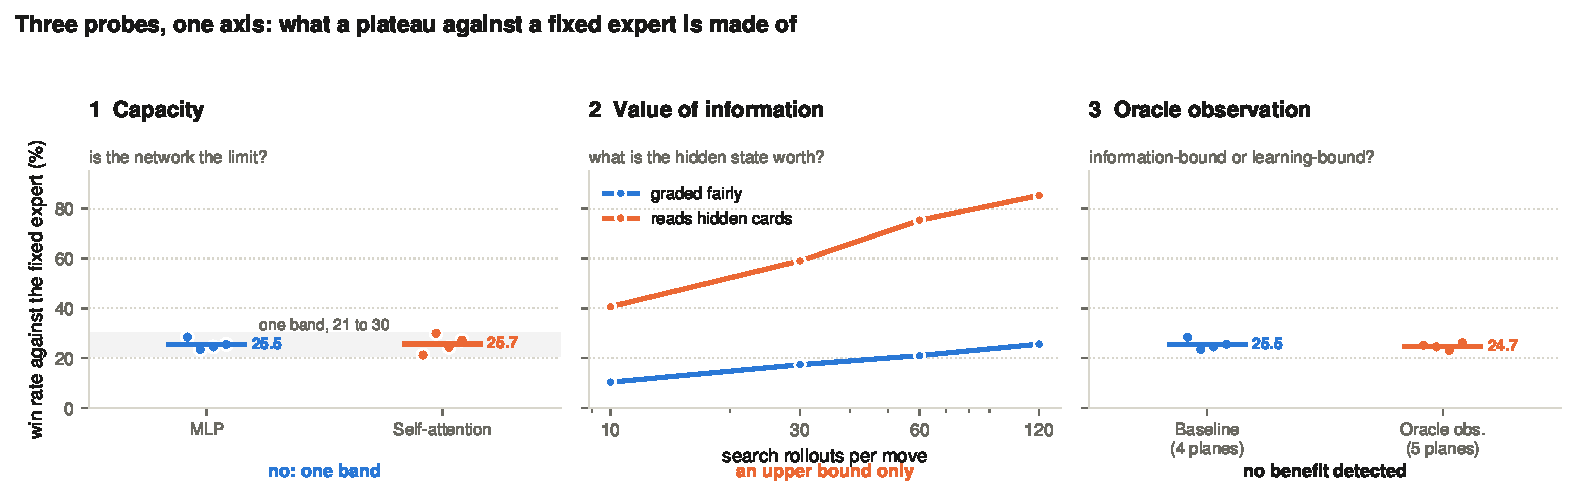
\includegraphics[width=0.96\linewidth]{fig1_three_probes.pdf}
  \caption{The three probes on one axis, win rate against the fixed expert. Dots are seeds, wide
  ticks are means.}
  \label{fig:probes}
\end{figure}

\paragraph{Probe 1: capacity.} Train the identical recipe with different encoders. A plain MLP
averages 25.5 percent over four seeds and a self-attention encoder 25.7, with all eight seeds inside
21.2 to 30.0. Attention buys variance, not mean, at roughly twelve times the wall-clock cost, so the
network is not the binding constraint.

\paragraph{Probe 2: the value of information, as an upper bound.} Run a determinized search
\citep{pimc,ismcts} graded fairly, then as an oracle handed the true hidden cards. Fair search
reaches 10.3 percent at 10 rollouts and 25.6 at 120; the oracle variant reaches 40.7 and 85.3 on
identical budgets. The gap bounds what the hidden information is worth but does not price it,
because oracle access also removes strategy fusion \citep{strategyfusion}, the reason determinized
search misjudges states it cannot distinguish and the motivation for belief-based methods
\citep{rebel}.

\paragraph{Probe 3: the oracle-observation learner.} Retrain the identical recipe with the hidden
state appended to the observation and change nothing else, putting the question to the learner
rather than to a search agent. Handed the opponent's hand outright, it reaches \ORACLEOBSMEAN{}
percent across \ORACLEOBSN{} seeds against a 25.5 baseline, and its range (23.1 to 26.2) sits
\emph{inside} the baseline's (23.5 to 28.4). Four seeds cannot prove the absence of an effect; what
they rule out is an effect large enough to explain the plateau.

Two details decide whether this probe measures what it claims. PettingZoo's own
\texttt{opponents\_hand\_visible} flag does \emph{not} supply the opponent's hand: it exposes an
``unknown cards'' plane that is nearly the complement of one's own hand and holds 41 cards on a
fresh deal against the opponent's 10. We verified our plane against engine ground truth at 1{,}200
decision points before spending compute. And since the curriculum's opponents read observations from
the same environment, we trim each opponent's input to the width its own network was trained on, so
the extra plane reaches the learner alone.

\section{Reading both halves together}

The atlas places Gin Rummy at 30.1 bits, within 4 of the two-player ceiling, so the agent is graded
in a genuinely information-rich game rather than a thin one. The probes then say it is not held back
by that information: capacity is not the limit, the subset argument puts parity inside the learner's
own information, and handing over the hidden state changes nothing measurable. The effort belongs in
optimisation, reward and curriculum, not in belief modelling.

\paragraph{When no strong reference exists.} Most domains have no hand-codable expert. In descending
order of what they buy: the strongest available heuristic, frozen, reported with its saturation
point; a frozen pool with a fixed Elo anchor; a snapshotted checkpoint promoted to reference and
never updated; or, best where possible, a reference deliberately built on a subset of the learner's
observation, which makes parity provably reachable by construction. Equilibrium baselines
\citep{cfr,nfsp,deepcfr} give an absolute reference where the game is small enough to solve.

\paragraph{Limitations.} One game, one expert, and an oracle bound confounded with strategy fusion.
The capacity probe covers the encoders we could train at scale. The closed forms count hands and
ignore public information. Bits are a property of the game and not of the difficulty of learning it:
we claim the two are routinely conflated, not that they are unrelated. Reported spreads are ranges
over four seeds, not confidence intervals; with this many seeds an interval estimator
\citep{rliable} would be the honest next step.

\section{Conclusion}

Choosing a domain is a measurement problem and reading a plateau is a diagnostic one, and both are
usually settled by tradition. Eighty-eight games measured, three probes, one verdict: this agent is
learning-bound, in a game that genuinely hides a great deal.

\bibliographystyle{plainnat}
\begin{thebibliography}{99}

\bibitem[Kelidari et al.(2026)]{goldstandard}
Kelidari, N.; Haghi, M.; and Salmani, M. 2026. \newblock A Gold-Standard Study of What Makes a Lightweight Game-Playing Agent Strong. \newblock In \emph{Proceedings of the AAAI Conference on Artificial Intelligence and Interactive Digital Entertainment (AIIDE)}. arXiv:2607.06854.

\bibitem[Bakhtin et al.(2022)]{cicero}
Meta Fundamental AI Research Diplomacy Team (FAIR); Bakhtin, A.; Brown, N.; Dinan, E.; Farina, G.; Flaherty, C.; Fried, D.; Goff, A.; Gray, J.; Hu, H.; et al. 2022. Human-Level Play in the Game of \emph{Diplomacy} by Combining Language Models with Strategic Reasoning. \emph{Science} 378(6624): 1067-1074.

\bibitem[Agarwal et al.(2021)]{rliable}
Agarwal, R.; Schwarzer, M.; Castro, P.~S.; Courville, A.~C.; and Bellemare, M.~G. 2021. Deep Reinforcement Learning at the Edge of the Statistical Precipice. In \emph{Advances in Neural Information Processing Systems (NeurIPS)} 34.

\bibitem[Brown and Sandholm(2018)]{libratus}
Brown, N.; and Sandholm, T. 2018. Superhuman AI for Heads-up No-Limit Poker: Libratus Beats Top Professionals. \emph{Science} 359(6374): 418-424.

\bibitem[Brown and Sandholm(2019)]{pluribus}
Brown, N.; and Sandholm, T. 2019. Superhuman AI for Multiplayer Poker. \emph{Science} 365(6456): 885-890.

\bibitem[Brown et al.(2019)]{deepcfr}
Brown, N.; Lerer, A.; Gross, S.; and Sandholm, T. 2019. Deep Counterfactual Regret Minimization. In \emph{Proceedings of the 36th International Conference on Machine Learning (ICML)}, 793-802.

\bibitem[Brown et al.(2020)]{rebel}
Brown, N.; Bakhtin, A.; Lerer, A.; and Gong, Q. 2020. Combining Deep Reinforcement Learning and Search for Imperfect-Information Games. In \emph{Advances in Neural Information Processing Systems (NeurIPS)} 33.

\bibitem[Cowling et al.(2012)]{ismcts}
Cowling, P.~I.; Powley, E.~J.; and Whitehouse, D. 2012. Information Set Monte Carlo Tree Search. \emph{IEEE Transactions on Computational Intelligence and AI in Games} 4(2): 120-143.

\bibitem[Frank and Basin(1998)]{strategyfusion}
Frank, I.; and Basin, D. 1998. Search in Games with Incomplete Information: A Case Study Using Bridge Card Play. \emph{Artificial Intelligence} 100(1-2): 87-123.

\bibitem[Heinrich and Silver(2016)]{nfsp}
Heinrich, J.; and Silver, D. 2016. Deep Reinforcement Learning from Self-Play in Imperfect-Information Games. arXiv:1603.01121.

\bibitem[Lanctot et al.(2019)]{openspiel}
Lanctot, M.; Lockhart, E.; Lespiau, J.-B.; Zambaldi, V.; Upadhyay, S.; P\'{e}rolat, J.; Srinivasan, S.; Timbers, F.; Tuyls, K.; Omidshafiei, S.; et al. 2019. OpenSpiel: A Framework for Reinforcement Learning in Games. arXiv:1908.09453.

\bibitem[Li et al.(2020)]{suphx}
Li, J.; Koyamada, S.; Ye, Q.; Liu, G.; Wang, C.; Yang, R.; Zhao, L.; Qin, T.; Liu, T.-Y.; and Hon, H.-W. 2020. Suphx: Mastering Mahjong with Deep Reinforcement Learning. arXiv:2003.13590.

\bibitem[Schofield and Thielscher(2019)]{ggpii}
Schofield, M.; and Thielscher, M. 2019. General Game Playing with Imperfect Information. \emph{Journal of Artificial Intelligence Research} 66.

\bibitem[Markowitz et al.(2018)]{rbccomplexity}
Markowitz, J.; Gardner, R.~W.; and Llorens, A.~J. 2018. On the Complexity of Reconnaissance Blind Chess. arXiv:1811.03119.

\bibitem[Lyle et al.(2022)]{capacityloss}
Lyle, C.; Rowland, M.; and Dabney, W. 2022. Understanding and Preventing Capacity Loss in Reinforcement Learning. In \emph{International Conference on Learning Representations (ICLR)}.

\bibitem[Rebstock et al.(2019)]{policyinference}
Rebstock, D.; Solinas, C.; Buro, M.; and Sturtevant, N.~R. 2019. Policy Based Inference in Trick-Taking Card Games. In \emph{IEEE Conference on Games (CoG)}.

\bibitem[Cover and Thomas(2006)]{coverthomas}
Cover, T.~M.; and Thomas, J.~A. 2006. \newblock \emph{Elements of Information Theory}, 2nd ed. \newblock Hoboken, NJ: Wiley-Interscience.

\bibitem[Howard(1966)]{voi}
Howard, R.~A. 1966. \newblock Information Value Theory. \newblock \emph{IEEE Transactions on Systems Science and Cybernetics} 2(1): 22--26.

\bibitem[Jacobs and Wallach(2021)]{measurementfairness}
Jacobs, A.~Z.; and Wallach, H. 2021. Measurement and Fairness. In \emph{Proceedings of the 2021 ACM Conference on Fairness, Accountability, and Transparency (FAccT)}, 375-385.

\bibitem[Raji et al.(2021)]{wholeworld}
Raji, I.~D.; Bender, E.~M.; Paullada, A.; Denton, E.; and Hanna, A. 2021. AI and the Everything in the Whole Wide World Benchmark. In \emph{Proceedings of the NeurIPS Track on Datasets and Benchmarks}.

\bibitem[Long et al.(2010)]{pimc}
Long, J.~R.; Sturtevant, N.~R.; Buro, M.; and Furtak, T. 2010. Understanding the Success of Perfect Information Monte Carlo Sampling in Game Tree Search. In \emph{Proceedings of the 24th AAAI Conference on Artificial Intelligence (AAAI)}, 134-140.

\bibitem[Ng et al.(1999)]{shaping}
Ng, A.~Y.; Harada, D.; and Russell, S. 1999. Policy Invariance under Reward Transformations: Theory and Application to Reward Shaping. In \emph{Proceedings of the 16th International Conference on Machine Learning (ICML)}, 278-287.

\bibitem[Schulman et al.(2017)]{ppo}
Schulman, J.; Wolski, F.; Dhariwal, P.; Radford, A.; and Klimov, O. 2017. Proximal Policy Optimization Algorithms. arXiv:1707.06347.

\bibitem[Silver et al.(2018)]{alphazero}
Silver, D.; Hubert, T.; Schrittwieser, J.; Antonoglou, I.; Lai, M.; Guez, A.; Lanctot, M.; Sifre, L.; Kumaran, D.; Graepel, T.; et al. 2018. A General Reinforcement Learning Algorithm that Masters Chess, Shogi, and Go through Self-Play. \emph{Science} 362(6419): 1140-1144.

\bibitem[Terry et al.(2021)]{pettingzoo}
Terry, J.~K.; Black, B.; Grammel, N.; Jayakumar, M.; Hari, A.; Sullivan, R.; Santos, L.; Perez, R.; Horsch, C.; Dieffendahl, C.; et al. 2021. PettingZoo: Gym for Multi-Agent Reinforcement Learning. In \emph{Advances in Neural Information Processing Systems (NeurIPS)} 34.

\bibitem[Zha et al.(2020)]{rlcard}
Zha, D.; Lai, K.-H.; Huang, S.; Cao, Y.; Reddy, K.; Vargas, J.; Nguyen, A.; Wei, R.; Guo, J.; and Hu, X. 2020. RLCard: A Platform for Reinforcement Learning in Card Games. In \emph{Proceedings of the 29th International Joint Conference on Artificial Intelligence (IJCAI)}, Demo Track.

\bibitem[Zha et al.(2021)]{douzero}
Zha, D.; Xie, J.; Ma, W.; Zhang, S.; Lian, X.; Hu, X.; and Liu, J. 2021. DouZero: Mastering DouDizhu with Self-Play Deep Reinforcement Learning. In \emph{Proceedings of the 38th International Conference on Machine Learning (ICML)}, 12333-12344.

\bibitem[Zinkevich et al.(2007)]{cfr}
Zinkevich, M.; Johanson, M.; Bowling, M.; and Piccione, C. 2007. Regret Minimization in Games with Incomplete Information. In \emph{Advances in Neural Information Processing Systems (NeurIPS)} 20.

\end{thebibliography}


\end{document}
